% Drawing 83/01-6 -- folder 83, batch 01, archive page 15 (PDF page 16).
% Transcription: un réseau de faces de l'icosaèdre autour de $u$ et $u_0$, sommets marqués $v_1$, $v_3'$, $v_4'$, $v_2$, $v_6'$, $v_3$, $v_4$, $v_2'$, $v_1'$ ; une face hachurée.
% Kind: net of icosahedron faces around two vertices. Method 2 (schematic redraw from the facsimile). Status: partial.
% Notes: Faces of the icosahedron around u (centre) and u_0 (top): the upper triangles A-B-C and A-D-C with heavy edges, the left face; below, the fan of triangles around the centre and the bottom vertex. The hatched face is the triangle u_0 - centre - right vertex. The vertex labels are placed as read on the crop (v'_4, v'_3, v_1, v_2, v'_6, v'_2, v_3, v_4, v'_1); the lower edges are a schematic reading of overlapping strokes.
% Coordinates: 1 unit = 1 mm = 1/100 of the crop width (bbox in page fractions: [0.45, 0.66, 0.68, 0.83]).
% Redrawn by Claude (claude-opus-5-5), issue #73, 2026-11-07; not checked by a human; not compiled (no TeX in the session).
% Rights: reproduces part of the work -- behind RENDER_TRANSCRIPTS, never published by itself.
\documentclass[tikz,border=3pt]{standalone}
\usepackage{amsmath,amssymb}
\usetikzlibrary{patterns,arrows.meta}
\tikzset{pencil/.style={black!45}, struck/.style={black!35}, mark/.style={circle,draw,inner sep=1.3pt}, pt/.style={circle,fill,inner sep=0.9pt}, opt/.style={circle,draw,fill=white,inner sep=1.1pt}}
\begin{document}
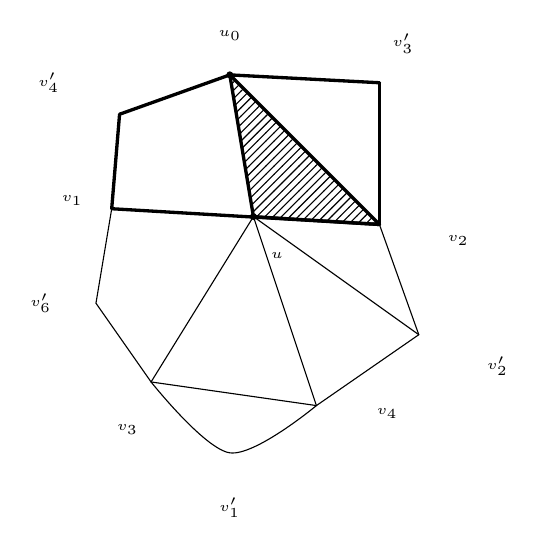
\begin{tikzpicture}[x=1mm,y=1mm,line cap=round,line join=round,font=\scriptsize]
\draw[very thick] (40,-37) -- (59,-38);
\draw[very thick] (59,-38) -- (59,-56);
\draw[very thick] (40,-37) -- (59,-56);
\draw[very thick] (40,-37) -- (43,-55);
\draw[very thick] (43,-55) -- (59,-56);
\draw[very thick] (25,-54) -- (59,-56);
\draw[very thick] (26,-42) -- (40,-37);
\draw[very thick] (25,-54) -- (26,-42);
\draw (25,-54) -- (43,-55);
\draw (25,-54) -- (23,-66);
\draw (23,-66) -- (30,-76);
\draw (43,-55) -- (30,-76);
\draw (43,-55) -- (51,-79);
\draw (30,-76) -- (51,-79);
\draw (59,-56) -- (64,-70);
\draw (64,-70) -- (51,-79);
\draw (43,-55) -- (64,-70);
\draw plot[smooth, tension=0.55] coordinates {(30,-76) (40,-85) (51,-79)};
\fill[pattern=north east lines] (40,-37) -- (43,-55) -- (59,-56) -- cycle;
\node[pt] at (40,-37) {};
\node[pt] at (43,-55) {};
\node[inner sep=1pt] at (40,-32) {\tiny $u_0$};
\node[inner sep=1pt] at (46,-60) {\tiny $u$};
\node[inner sep=1pt] at (17,-38) {\tiny $v'_4$};
\node[inner sep=1pt] at (62,-33) {\tiny $v'_3$};
\node[inner sep=1pt] at (20,-53) {\tiny $v_1$};
\node[inner sep=1pt] at (69,-58) {\tiny $v_2$};
\node[inner sep=1pt] at (16,-66) {\tiny $v'_6$};
\node[inner sep=1pt] at (74,-74) {\tiny $v'_2$};
\node[inner sep=1pt] at (27,-82) {\tiny $v_3$};
\node[inner sep=1pt] at (60,-80) {\tiny $v_4$};
\node[inner sep=1pt] at (40,-92) {\tiny $v'_1$};
\end{tikzpicture}
\end{document}
